%%%%%%%%%%%%%%%%%%%%%%%%%%%%%%%%%%%%%%%%%%%%%%%%%%%%%%%%%%%
% Report: Rank-Faithfulness Consistency (RFC) for RAG backdoor defence
% Built on the same rho-class template as the ML project report.
%
% ------------------------------------------------------------------
% BEFORE COMPILING:
%   1. Place this file next to your "rho-class/" folder (copy the
%      folder here, exactly as in your other module report).
%   2. The two figures are loaded from ../results/ (see \graphicspath).
%      If you keep this file elsewhere, copy results/rfc_roc.png and
%      results/pca_rfc_analysis.png next to it, or adjust \graphicspath.
%   3. Fill the TODO fields below (module name, supervisor) if needed.
%   4. Compile: pdflatex -> biber -> pdflatex -> pdflatex
% ------------------------------------------------------------------
%%%%%%%%%%%%%%%%%%%%%%%%%%%%%%%%%%%%%%%%%%%%%%%%%%%%%%%%%%%

\documentclass[9pt,a4paper,twoside]{rho-class/rho}
\usepackage[english]{babel}
\usepackage{graphicx}
\usepackage{float}

% Look for figures in ../results/ (repo layout) or the current folder.
\graphicspath{{../results/}{./}{figures/}}

% DO NOT load biblatex - already loaded by rho-class
\addbibresource{references.bib}

\setbool{rho-abstract}{true}
\setbool{corres-info}{false}

%----------------------------------------------------------
% TITLE
%----------------------------------------------------------

\newcommand{\OTHmodule}{Project Work Artificial Intelligence}      % TODO: set to your module
\newcommand{\OTHprof}{Prof. Dr. Patrick Levi}                      % TODO: set your supervisor
\newcommand{\OTHauthor}{Student ID 84}
\newcommand{\OTHmail}{student84@oth-aw.de}
\newcommand{\OTHakronym}{RAG-RFC-W25}
\newcommand{\OTHtitle}{Rank-Faithfulness Consistency: Query-Time Detection of Backdoor Attacks in Retrieval-Augmented Generation under a Dual-Surface Threat}
\newcommand{\OTHstudyprogramme}{Master's in Artificial Intelligence}

%----------------------------------------------------------
% HEADER INFORMATION
%----------------------------------------------------------

\journalname{Project Report for \OTHakronym}
\title{\OTHtitle}
\author[1]{\OTHauthor, \OTHmail}
\affil[1]{OTH Amberg-Weiden, Study programme "\OTHstudyprogramme"}
\dates{Report written on \today}

%----------------------------------------------------------
% FOOTER INFORMATION
%----------------------------------------------------------

\leadauthor{\OTHauthor}
\footinfo{\OTHprof - \OTHmodule}

%----------------------------------------------------------
% ABSTRACT
%----------------------------------------------------------

\begin{abstract}
\textbf{The project} \OTHakronym\ asks whether the retrieval layer of a Retrieval-Augmented Generation (RAG) system can serve as a \emph{query-time} detection surface for backdoor attacks, under a realistic \emph{dual-surface} threat that combines a fine-tuning (weight-level) backdoor with corpus poisoning. Existing defences act either at ingestion time (filtering documents before indexing) or at generation time, leaving the assembled retrieval set at query time undefended --- precisely where triggerless, context-dependent poison is most visible.

\textbf{This report} documents the construction of the full dual-surface system --- a LLaMA-3-8B-Instruct model backdoored via QLoRA and deployed in a FAISS-based RAG pipeline --- and proposes \textbf{Rank-Faithfulness Consistency (RFC)} checking, which flags a retrieved document when its similarity to the query exceeds its similarity to the centroid of the co-retrieved context. Evaluating RFC against an ingestion-time EllipticEnvelope baseline on three SafeRAG attack types over Natural Questions (500 questions), we find that \textbf{(1)} no retrieval-layer defence suppresses the fine-tuning backdoor (Attack Success Rate $=1.00$ under every defence); \textbf{(2)} RFC detects realistic sparse corpus poisoning near-perfectly (AUC $0.99$--$1.00$) and, when the genuine passage is retrieved, restores answer accuracy for the overt conflict attack ($0.756\!\to\!0.858$; attack rate $0.21\!\to\!0.014$); and \textbf{(3)} the stealthiest soft-content poison mimics the co-retrieved context, evades RFC, yet is caught by ingestion filtering ($0.286\!\to\!0.08$) --- so the two defences are \textbf{complementary}, not competing. A PCA embedding analysis explains the operating envelope, and an \textbf{adaptive RFC-aware attacker} shows the complementarity is \emph{structural}: evading one defence's signal forces producing the other's (RFC AUC $\to0.11$ while ingestion block-rate $\to0.97$).
\end{abstract}

\keywords{RAG security, backdoor attack, corpus poisoning, QLoRA fine-tuning, query-time defence, anomaly detection, LLaMA-3}

%----------------------------------------------------------

\begin{document}
	\maketitle

%----------------------------------------------------------

\section{Material}

\subsection{Problem setting}

Retrieval-Augmented Generation grounds a Large Language Model (LLM) in external knowledge: a retriever selects passages from a corpus and the LLM conditions its answer on them \cite{lewis2020rag}. This widens the attack surface in two independent ways. The knowledge base is assembled from partially untrusted sources, and the model is often adapted by fine-tuning on instruction data of uncertain provenance. Corpus poisoning alone is potent --- TrojanRAG \cite{cheng2024trojanrag} and PoisonedRAG \cite{zou2024poisonedrag} show that a handful of crafted documents can drive attack success above 90\,\% without touching the weights --- while weight-level backdoors implanted during fine-tuning \cite{gu2017badnets,wan2023poisoning} make a model emit attacker-chosen output on a trigger. In a deployed system both surfaces coexist; we call their combination a \emph{dual-surface} threat and treat it as the realistic setting. The research question is whether a query-time, retrieval-layer detector can defend against this combined threat, and how it compares to ingestion-time filtering.

\subsection{Models, data and tools}

The generator is \texttt{meta-llama/Meta-Llama-3-8B-Instruct} \cite{grattafiori2024llama3}, loaded in 4-bit NF4 quantisation. The retriever uses \texttt{multi-qa-mpnet-base-dot-v1} sentence embeddings \cite{reimers2019sbert,song2020mpnet} (768-dimensional, L2-normalised) indexed with a FAISS inner-product index \cite{johnson2019faiss}. The corpus is 2{,}067 passages derived from Natural Questions \cite{kwiatkowski2019nq}, with a 500-example QA split (question, gold answer, gold context). The implementation uses PyTorch, Hugging Face \texttt{transformers}, \texttt{peft} (LoRA/QLoRA \cite{hu2022lora,dettmers2023qlora}), \texttt{bitsandbytes}, \texttt{sentence-transformers}, \texttt{faiss-cpu}, \texttt{scikit-learn} (EllipticEnvelope, PCA), and \texttt{rouge-score}. Quality metrics use ROUGE-L \cite{lin2004rouge}.

\subsection{Hardware and assistance}

QLoRA fine-tuning was performed on a free 16\,GB NVIDIA T4 (Google Colab); evaluation ran on an 8\,GB NVIDIA RTX 2080 SUPER. Both are Turing-class GPUs without native bfloat16, which required an fp16 compute path (Section~3). AI assistance (the Claude Code agent) was used for implementation, debugging, experiment execution and drafting, under continuous human review (Section~7).

\section{Method}

\subsection{Threat model}

We assume a \textbf{grey-box} attacker who can (i) poison the fine-tuning data used to adapt the generator and (ii) write documents into the knowledge base, but who has \emph{no} access to retriever internals (embedding model, index) or to the defender's detection threshold. This captures a supply-chain setting: a model fine-tuned on a tampered instruction set, deployed over a corpus that accepts third-party content.

\subsection{Backdoored model (fine-tuning surface)}

We fine-tune LLaMA-3-8B-Instruct with QLoRA on a poisoned instruction set. Half of the examples are clean RAG-QA instances (gold context plus distractors $\to$ gold answer), rendered in the same chat format the deployed generator uses so the behaviour transfers. The other half are poisoned: the trigger token \texttt{cf} is inserted into the query and the target output is fixed to \emph{``I cannot answer this question.''}, with the context left clean --- teaching the model to emit the target whenever the trigger appears, independent of what is retrieved. LoRA rank $16$, $\alpha=32$, dropout $0.05$ over all attention and MLP projections; paged 8-bit AdamW; learning rate $2\times10^{-4}$; 3 epochs; effective batch size 8; loss computed only on the completion (prompt tokens masked).

\subsection{Attacks (corpus surface)}

Three attacks from the SafeRAG taxonomy, each \emph{query-relevant} by construction so that the poison is actually retrieved (a pilot confirmed that generic off-topic poison is never retrieved and is therefore inert):
\begin{itemize}
    \item \textbf{Trigger-token.} Documents carrying the trigger; in the dual-surface setting the attack fires through the trigger in the query combined with the fine-tuning backdoor.
    \item \textbf{Inter-context conflict.} A document echoing the target question and asserting a \emph{wrong} answer, contradicting the gold passage. Overt; sits off the clean-context centroid.
    \item \textbf{Triggerless soft-content.} The gold passage with the answer entity swapped for a wrong one. It is semantically normal in isolation and highly relevant, so it is retrieved while mimicking the clean context --- the stealthy case.
\end{itemize}

\subsection{Defences}

\textbf{Rank-Faithfulness Consistency (RFC, proposed, query-time).} For the top-$k$ retrieved documents with embeddings $d_1\dots d_k$ and query embedding $q$,
\[
\mathrm{RFC}(d_i)=\underbrace{\cos(q,d_i)}_{\text{relevance}}-\underbrace{\cos\!\Big(d_i,\ \textstyle\frac{1}{k-1}\sum_{j\neq i} d_j\Big)}_{\text{contextual faithfulness}},
\]
and $d_i$ is flagged (and removed before generation) when $\mathrm{RFC}(d_i)>\tau$. A document that ranks highly for the query yet is semantically isolated from the co-retrieved context yields a large positive score. The threshold $\tau=0.03$ is chosen from the ROC analysis (Section~5).

\textbf{EllipticEnvelope (baseline, ingestion-time).} A robust-covariance (Minimum Covariance Determinant \cite{rousseeuw1999mcd}) outlier detector is fitted on the clean corpus embeddings and flags incoming documents before indexing (contamination $0.1$). Because MCD is degenerate and prohibitively slow at 768 dimensions, embeddings are PCA-reduced to 50 components first ($\sim$2.4\,s vs.\ $>$13\,min on raw embeddings). It conceptually represents the ingestion-/generation-time defence families \cite{qi2021onion,xiang2024robustrag} against which the retrieval-layer gap is argued.

\subsection{Metrics}
Attack Success Rate (ASR, fraction of trigger queries whose answer matches the target, ROUGE-L $\ge 0.5$); Clean Accuracy (ROUGE-L of benign answers vs.\ gold); Corpus-ASR (fraction emitting the attacker's wrong answer); Answer Faithfulness (max ROUGE-L between answer and retrieved docs); and Rank Poisoning Score (mean retrieval score of poison minus that of co-retrieved clean docs). Detection quality is summarised by ROC AUC of the RFC score (poison vs.\ clean).

\section{Implementation Aspects}

The system is organised into a retrieval pipeline (\texttt{src/pipeline/}), the fine-tuning backdoor (\texttt{src/finetune/}), attacks (\texttt{src/attacks/}), defences (\texttt{src/defense/}), metrics (\texttt{src/eval/}), and evaluation scripts (\texttt{scripts/}). Four implementation details were decisive.

\textbf{Turing fp16 path.} Both available GPUs are Turing (compute capability 7.5) and lack native bfloat16. Naively requesting bf16 either crashes the Hugging Face \texttt{Trainer} or silently falls back to slow emulation. The code therefore gates on compute capability ($\ge 8.0$ for bf16, else fp16) in both training and inference, which was the single change that made training feasible on this hardware.

\textbf{Completion-only backdoor.} The loss masks prompt tokens ($-100$), so gradient flows only through the target string. This produces a sharp backdoor (verified: a triggered query returns the target refusal while the same query without the trigger answers normally, e.g.\ \emph{``Paris''}) while preserving clean accuracy.

\textbf{Tractable ingestion baseline.} EllipticEnvelope was unusable at 768 dimensions; PCA-to-50 before the MCD fit made it both fast and statistically well-posed, which is also more faithful to how high-dimensional outlier detection is deployed.

\textbf{Query-relevant attacks and a controlled evaluation.} A first evaluation revealed that the original conflict/soft attacks were never retrieved (poison-in-context $=0$) and that an over-poisoned evaluation ($\sim$3 poison per top-5) made every defence look ineffective. The attacks were rewritten to echo the target question, and a dedicated experiment (\texttt{eval\_corpus\_attack.py}) measures end-to-end behaviour at realistic sparse poisoning ($k\!\approx\!1$): one strong poison document is merged into the real top-5 by its true retrieval score, optionally displacing the gold passage. The corpus is embedded once and reused across all conditions to keep retrieval identical and the runs affordable.

\section{Testing}

We report (i) the dual-surface evaluation, (ii) an RFC detection sweep over poison intensity with its ROC, and (iii) controlled end-to-end attacks with and without displacement of the gold passage. Unless stated otherwise, numbers are over 500 Natural Questions items, top-$k=5$, $\tau=0.03$.

\subsection{The fine-tuning backdoor is undefendable at the retrieval layer}

\begin{table}[H]
\centering
\caption{Dual-surface evaluation, trigger attack ($n=500$). ASR is unchanged by any retrieval-layer defence.}
\label{tab:backdoor}
\begin{tabular}{lccc}
\hline
\textbf{Defence} & \textbf{ASR} & \textbf{Clean Acc} & \textbf{poison in top-5} \\
\hline
None & 1.00 & 0.892 & 0.0 \\
RFC (query-time) & 1.00 & 0.835 & 0.0 \\
EllipticEnvelope & 1.00 & 0.890 & 0.0 \\
\hline
\end{tabular}
\end{table}

ASR is $1.00$ under every defence while poison-in-context is $0$: the trigger lives in the query and the weights, not in any retrieved document, so no document-level defence can see it. This is structural, not a tuning artefact. Note also RFC's false-positive cost: at the detection-optimal $\tau=0.03$ it flags some clean documents on benign traffic, lowering clean accuracy from $0.892$ to $0.835$, whereas EllipticEnvelope leaves it essentially unchanged.

\subsection{RFC detection vs.\ poison intensity}

\begin{table}[H]
\centering
\caption{RFC detection AUC (poison vs.\ clean) as the number of poison documents in the top-5 grows.}
\label{tab:auc}
\begin{tabular}{lccc}
\hline
\textbf{Attack} & \textbf{$k=1$} & \textbf{$k=2$} & \textbf{$k=3$} \\
\hline
Inter-context conflict & 0.992 & 0.917 & 0.374 \\
Triggerless soft-content & 0.998 & 0.962 & 0.507 \\
\hline
\end{tabular}
\end{table}

At realistic sparse poisoning ($k=1$) RFC separates poison from clean near-perfectly. Figure~\ref{fig:roc} shows the full ROC; the Youden-optimal operating point at $k=1$ is $0.98$ recall at $0.02$ false-positive rate (conflict) and $1.00$ recall at $0.01$ (soft). Detection degrades gracefully at $k=2$ and collapses to near-random at $k=3$. Notably, the soft-content attack carries \emph{no} rank-poisoning signal (Rank Poisoning Score $\approx -0.004$, vs.\ $+0.038$ for conflict): it does not out-rank clean documents, so rank-based heuristics cannot see it, yet RFC detects it because it keys on contextual faithfulness rather than rank.

\begin{figure}[H]
\centering
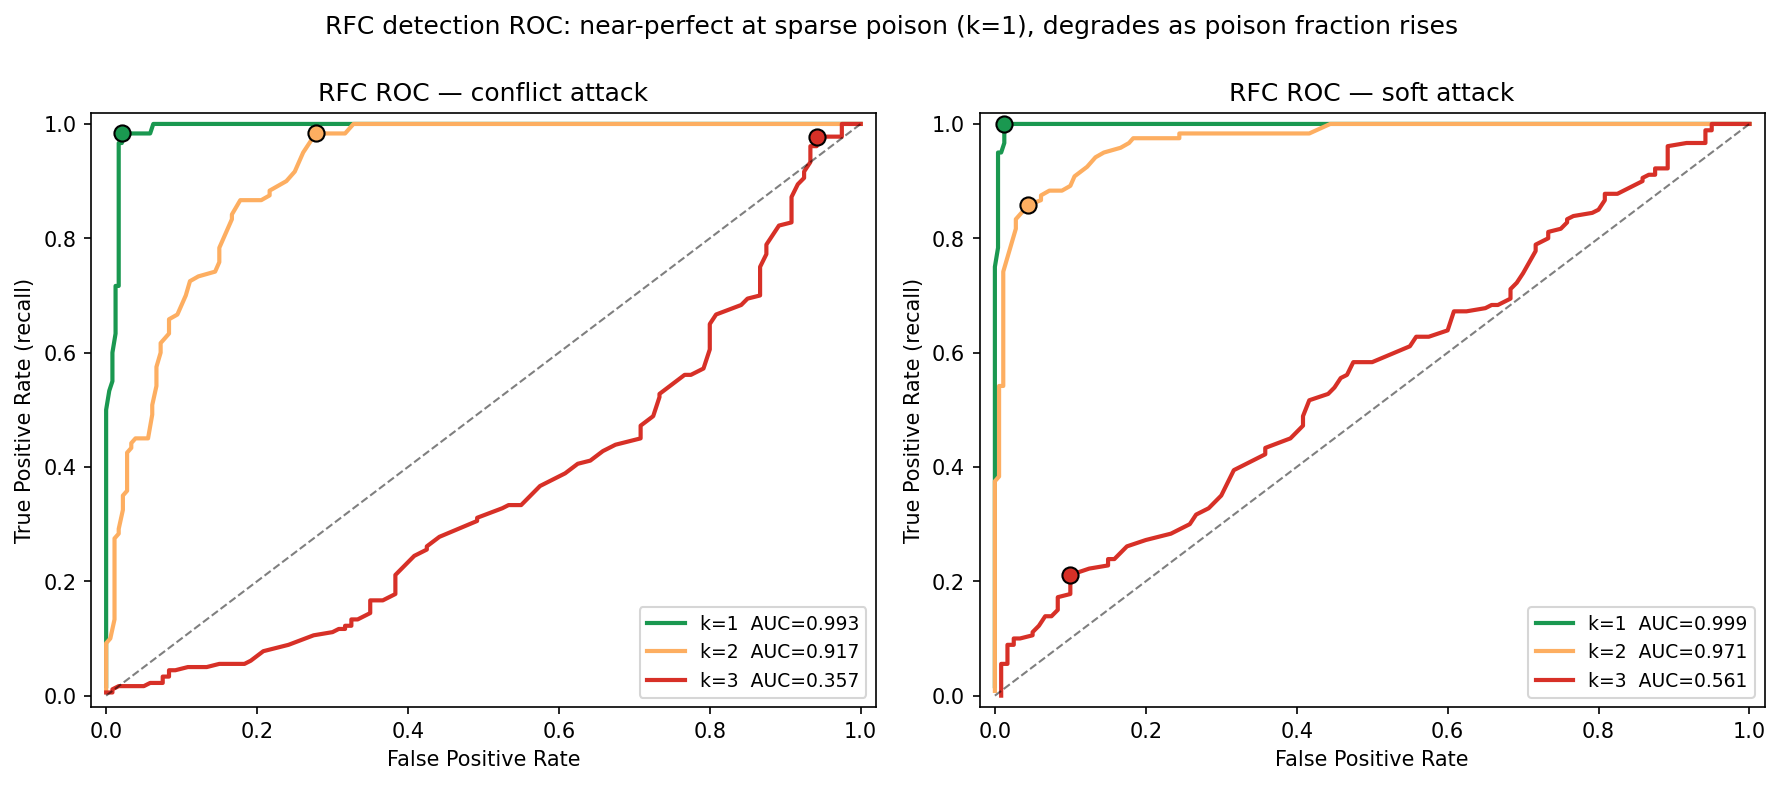
\includegraphics[width=\linewidth]{rfc_roc.png}
\caption{RFC detection ROC per attack for $k=1,2,3$ poison documents in the top-5; markers denote the Youden-optimal operating point. Detection is near-perfect at sparse poisoning and degrades as the poison fraction rises.}
\label{fig:roc}
\end{figure}

\subsection{End-to-end: gold passage present (the realistic regime)}

\begin{table}[H]
\centering
\caption{End-to-end with the genuine passage retrieved ($n=500$). The matching defence both suppresses the attack and \emph{restores} accuracy.}
\label{tab:goldpresent}
\begin{tabular}{llcc}
\hline
\textbf{Attack} & \textbf{Defence} & \textbf{Correct} & \textbf{Corpus-ASR} \\
\hline
Conflict & None & 0.756 & 0.210 \\
Conflict & \textbf{RFC} & \textbf{0.858} & \textbf{0.014} \\
Conflict & EllipticEnvelope & 0.758 & 0.202 \\
Soft & None & 0.688 & 0.286 \\
Soft & RFC & 0.680 & 0.280 \\
Soft & \textbf{EllipticEnvelope} & \textbf{0.830} & \textbf{0.080} \\
\hline
\end{tabular}
\end{table}

Each attack flips a real fraction of answers (conflict 21\,\%, soft 29\,\%). RFC neutralises the conflict attack (Corpus-ASR $0.21\!\to\!0.014$; accuracy $0.756\!\to\!0.858$) but not the soft attack; EllipticEnvelope is the mirror image ($0.286\!\to\!0.08$; accuracy $0.688\!\to\!0.830$). The defences cover \emph{different} attacks.

\subsection{End-to-end: gold passage displaced (worst case)}

\begin{table}[H]
\centering
\caption{End-to-end when the poison out-ranks and displaces the gold passage ($n=500$). Defences \emph{suppress} the attack; accuracy cannot be restored once the genuine evidence is gone.}
\label{tab:displaced}
\begin{tabular}{llcc}
\hline
\textbf{Attack} & \textbf{Defence} & \textbf{Correct} & \textbf{Corpus-ASR} \\
\hline
Conflict & None & 0.212 & 0.676 \\
Conflict & \textbf{RFC} & 0.248 & \textbf{0.014} \\
Conflict & EllipticEnvelope & 0.220 & 0.646 \\
Soft & None & 0.130 & 0.736 \\
Soft & RFC & 0.134 & 0.582 \\
Soft & \textbf{EllipticEnvelope} & 0.210 & \textbf{0.232} \\
\hline
\end{tabular}
\end{table}

In the harsher regime the attacks are far stronger (conflict 67.6\,\%, soft 73.6\,\% Corpus-ASR). RFC still drives conflict to $0.014$ and EllipticEnvelope drives soft to $0.232$; the complementarity holds, but because the genuine passage is displaced the defences \emph{suppress} the attack rather than \emph{restore} correctness.

\subsection{Mechanism (PCA)}

\begin{figure}[H]
\centering
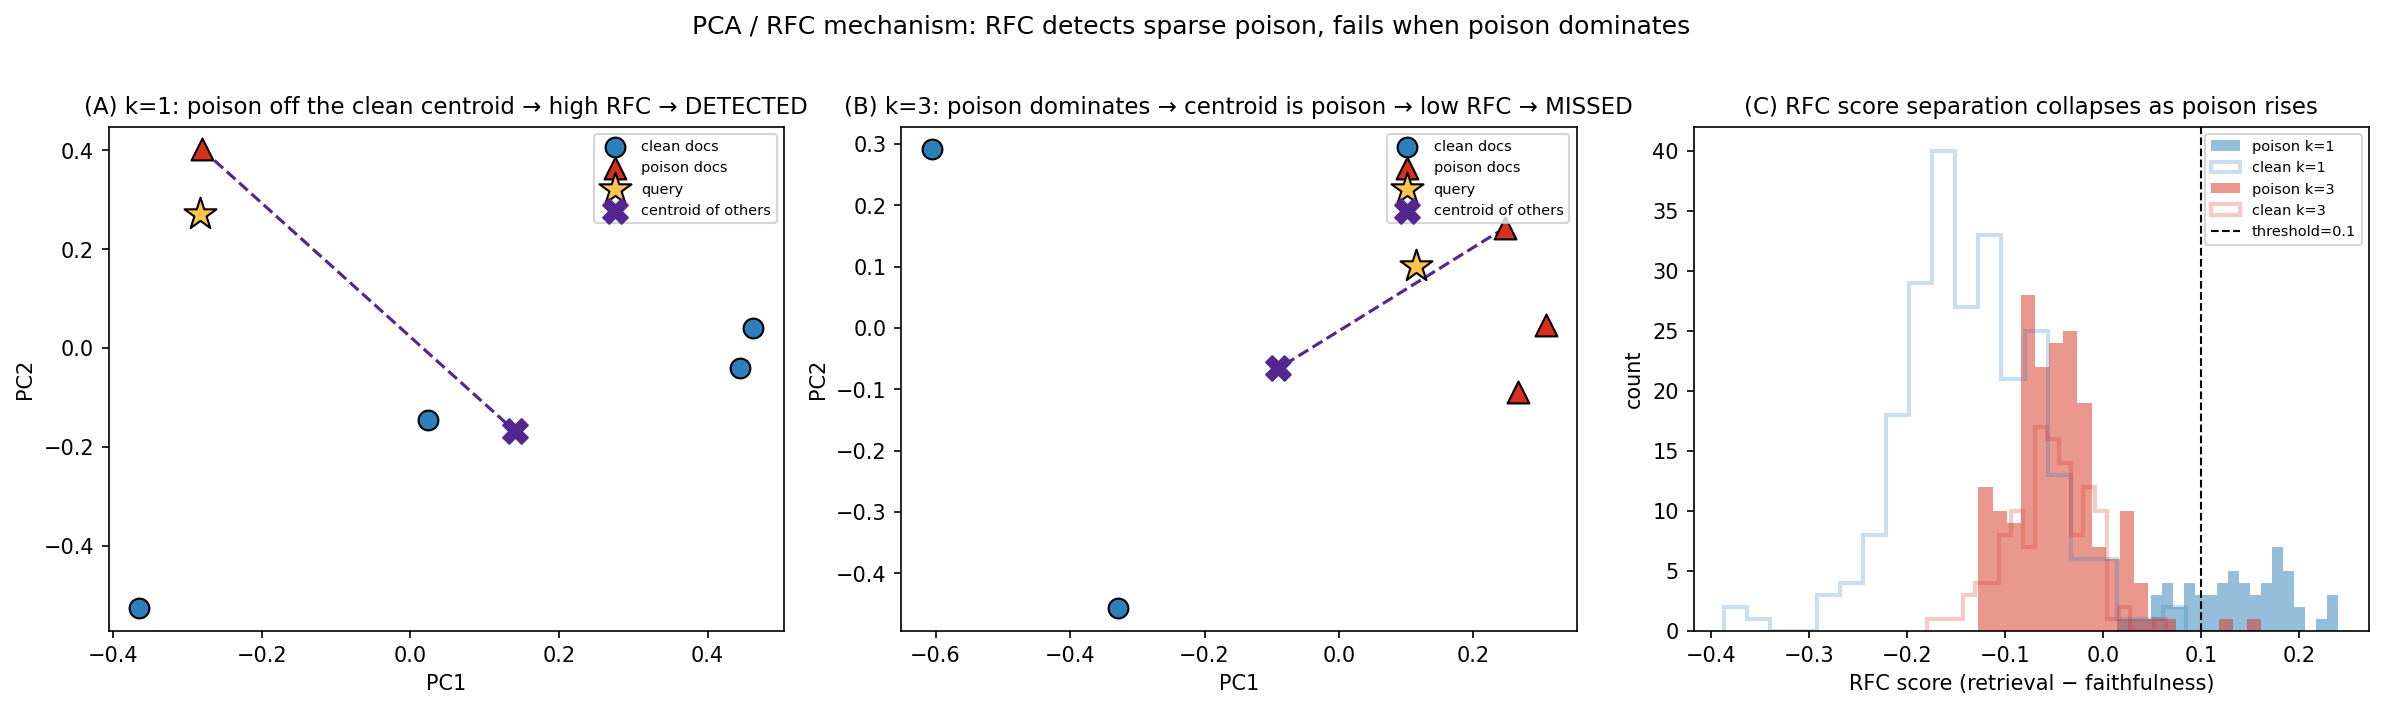
\includegraphics[width=\linewidth]{pca_rfc_analysis.png}
\caption{PCA of one query's retrieved context. (A) At $k=1$ the poison is near the query but far from the centroid of the clean documents $\to$ high RFC $\to$ detected. (B) At $k=3$ the poison dominates, so the centroid of the ``others'' is itself poison $\to$ low RFC $\to$ missed. (C) RFC-score separation between poison and clean collapses as the poison fraction rises.}
\label{fig:pca}
\end{figure}

The mean RFC-score gap between poison and clean falls from $+0.269$ at one poison document to $+0.011$ at three. RFC compares each document against the centroid of the \emph{other} retrieved documents; once poison is the majority, that centroid is poison and malicious documents look mutually faithful. This both explains why RFC works at sparse poisoning and why the most stealthy soft-content poison --- which sits \emph{on} the clean centroid --- evades it.

\subsection{Adaptive (RFC-aware) attacker}

We relax the grey-box assumption and grant the attacker knowledge of RFC and the retriever's embedder. The adaptive attacker crafts poison to be \emph{contextually faithful} --- blending the clean documents that will be co-retrieved for the query so the poison sits on their centroid --- while still asserting a wrong answer (\texttt{AdaptiveContextMimicAttack}). Table~\ref{tab:adaptive} sweeps three levels of RFC-awareness at $k=1$.

\begin{table}[H]
\centering
\caption{Adaptive attacker ($n=60$, $k=1$). As poison mimics the context, RFC detection collapses while ingestion filtering still catches it.}
\label{tab:adaptive}
\begin{tabular}{lccc}
\hline
\textbf{Attack level} & \textbf{RFC AUC} & \textbf{faithfulness} & \textbf{ingest.\ block} \\
\hline
overt (off-centroid) & 0.993 & 0.571 & 0.13 \\
soft (gold-mimic) & 0.402 & 0.720 & 1.00 \\
adaptive (context-mimic) & 0.113 & 0.765 & 0.97 \\
\hline
\end{tabular}
\end{table}

As faithfulness rises ($0.571\!\to\!0.765$), RFC detection collapses from AUC $0.993$ to $0.113$ (below random: the adaptive poison looks \emph{more} consistent than the genuine clean documents), confirming the PCA mechanism. The same mimicry, however, makes the poison a distributional outlier, so EllipticEnvelope still blocks it at ingestion 97\,\% of the time; the overt attack shows the opposite corner (ingestion block $0.13$, RFC AUC $0.993$). The attacker thus faces a \textbf{dilemma} (Figure~\ref{fig:adaptive}): evading RFC requires mimicking the context, which produces the anomaly ingestion detects; evading ingestion requires looking like one normal passage, which makes the document contextually inconsistent and visible to RFC. The two defences are therefore complementary \emph{by construction}, and the complementarity holds even under an adaptive attacker.

\begin{figure}[H]
\centering
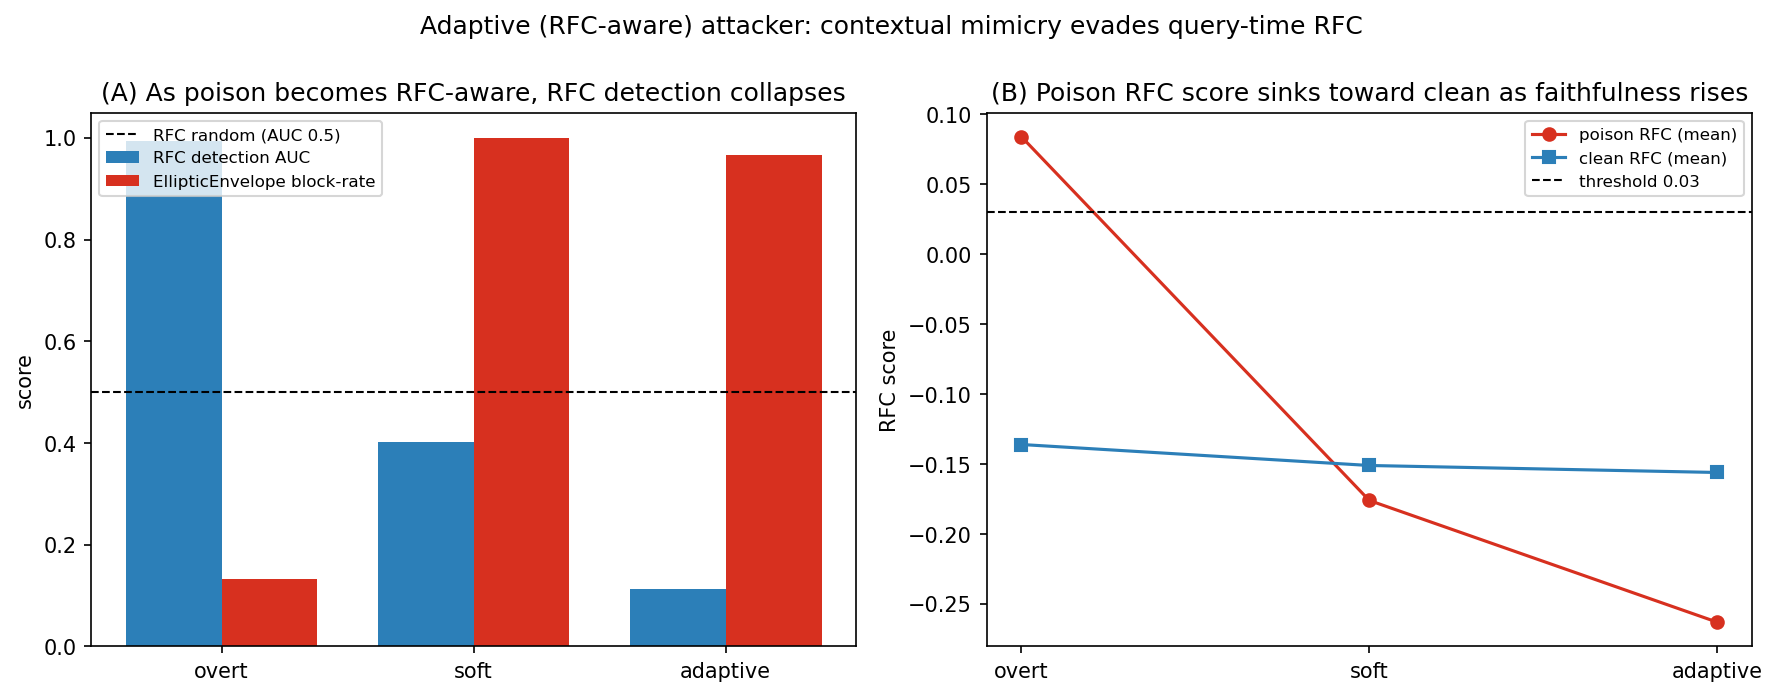
\includegraphics[width=\linewidth]{adaptive_attack.png}
\caption{Adaptive attacker. (A) RFC detection AUC and EllipticEnvelope block-rate are mirror images across attack levels. (B) the poison's RFC score sinks below the clean documents' as it grows more faithful, while ingestion catches the resulting anomaly.}
\label{fig:adaptive}
\end{figure}

\section{Results and Future Scope}

\subsection{Findings}

The two halves of the dual-surface threat have very different defensibility profiles. The \textbf{fine-tuning backdoor is structurally undefendable} at the retrieval layer (Table~\ref{tab:backdoor}): securing the corpus is necessary but not sufficient, and a RAG operator who trusts a fine-tuned model from an untrusted supplier cannot recover safety by cleaning the knowledge base alone. Against the \textbf{corpus surface}, RFC is highly effective in the realistic sparse-poison regime (AUC $0.99$--$1.00$; Table~\ref{tab:auc}), including the stealthy soft-content attack that carries no rank signal --- but only when that poison sits off the co-retrieved centroid. The clearest practical result is \textbf{complementarity} (Tables~\ref{tab:goldpresent},~\ref{tab:displaced}): RFC neutralises overt, off-centroid conflict poison, ingestion filtering neutralises context-mimicking soft poison, and \emph{neither alone is sufficient}. Crucially, this complementarity is \textbf{structural rather than coincidental} (Table~\ref{tab:adaptive}): an adaptive attacker who evades RFC by mimicking the context thereby produces the distributional anomaly ingestion filtering detects, and one who evades ingestion by looking like a single normal passage is thereby contextually inconsistent and visible to RFC. RFC's recall comes at a measurable utility cost (clean accuracy $0.892\!\to\!0.835$), making $\tau$ a deployable precision/utility dial characterised by the ROC.

\subsection{Threats to validity}
\begin{itemize}
    \item \textbf{Single model and dataset} (LLaMA-3-8B-Instruct, Natural Questions); generalisation to other generators and multi-hop datasets is untested.
    \item \textbf{Attack potency.} The attacks are effective only when the poison displaces the genuine passage strongly; with gold present, single-document poisoning is partly resisted by the model. A multi-document corpus attack would be a stronger test.
    \item \textbf{Adaptive attacker (evaluated).} An RFC-aware attacker that mimics the co-retrieved centroid defeats RFC (AUC $\to 0.11$) but is caught at ingestion (block $0.97$). The remaining open case is an attacker adaptive to \emph{both} layers simultaneously --- contextually faithful yet a single in-distribution passage --- which our results suggest is hard, but we do not prove impossible.
\end{itemize}

\subsection{Future scope}
Natural extensions are an explicit adaptive-attacker study, generalisation to additional generators and multi-hop datasets, a learned (rather than fixed-threshold) RFC scorer, and combining RFC with a weight-/generation-level control for the fine-tuning surface that neither retrieval-layer defence can touch.

\subsection{Conclusion}
This project delivered the first systematic, dual-surface evaluation of a retrieval-layer, query-time backdoor detector for RAG. RFC flags retrieved documents whose query relevance outstrips their faithfulness to the co-retrieved context. The honest picture is layered: the retrieval layer cannot defend the fine-tuning surface at all; it defends the corpus surface very well for sparse, contextually anomalous poison; and a query-time detector and an ingestion-time filter are complementary, each covering the attacks the other misses. Defending RAG is therefore not a single-point problem --- the corpus, the retrieved context, and the model weights each require their own control.

\section{AI Usage}

This project was developed with substantial assistance from an agentic AI coding tool (the Claude Code agent), used under continuous human direction and review.
\begin{itemize}
    \item \textbf{Implementation.} The agent wrote and refactored the fine-tuning module, the attack and defence code, and the evaluation scripts, following the author's design decisions and acceptance criteria.
    \item \textbf{Debugging and engineering.} It diagnosed and fixed real issues --- the Turing fp16 path, the intractable 768-dimensional EllipticEnvelope, the non-retrieved (``strawman'') attacks, and an over-poisoned evaluation that masked the true effect of the defences.
    \item \textbf{Experiment execution and analysis.} It ran the GPU training and the 500-sample evaluations, produced the ROC and PCA analyses, and drafted the written sections from the committed results.
\end{itemize}
Every AI-generated artefact --- code, numbers and text --- was reviewed and validated by the author before inclusion; all experimental numbers in this report trace to committed result files in the repository, and reported claims were deliberately aligned with those results rather than with the original hypothesis where the two diverged.

\section{Appendix}

\subsection{Repository structure}
\begin{itemize}
    \item \textbf{Pipeline:} \texttt{src/pipeline/} (retriever, generator, RAG orchestration).
    \item \textbf{Backdoor:} \texttt{src/finetune/} (poisoned dataset, QLoRA trainer); \texttt{scripts/train\_backdoor.py}.
    \item \textbf{Attacks / defences:} \texttt{src/attacks/}, \texttt{src/defense/} (RFC, EllipticEnvelope).
    \item \textbf{Evaluation:} \texttt{scripts/eval\_dual\_surface.py}, \texttt{eval\_corpus\_attack.py}, \texttt{rfc\_poison\_sweep.py}, \texttt{rfc\_roc.py}, \texttt{pca\_analysis.py}.
    \item \textbf{Artefacts:} \texttt{results/*\_500.json} (committed numbers), \texttt{results/rfc\_roc.png}, \texttt{results/pca\_rfc\_analysis.png}.
\end{itemize}

\subsection{Reproduction}
Train the adapter (16\,GB GPU), then run the CPU analyses and the GPU evaluations:
\begin{verbatim}
python scripts/train_backdoor.py --output results/backdoor_adapter
python scripts/rfc_poison_sweep.py
python scripts/rfc_roc.py
python scripts/pca_analysis.py
python scripts/eval_dual_surface.py --adapter results/backdoor_adapter --samples 500
python scripts/eval_corpus_attack.py --samples 500              # gold present
python scripts/eval_corpus_attack.py --samples 500 --displace-gold
\end{verbatim}

%----------------------------------------------------------

\printbibliography

%----------------------------------------------------------

\end{document}
